\documentclass[tikz]{standalone}
\usepackage{framed}
\usepackage{amsmath} 
\usepackage{amsfonts}
\DeclareMathOperator{\f}{f}
\usepackage{xcolor}

\usetikzlibrary{shadows.blur}
\usetikzlibrary{arrows}
\usetikzlibrary{positioning}

\begin{document}
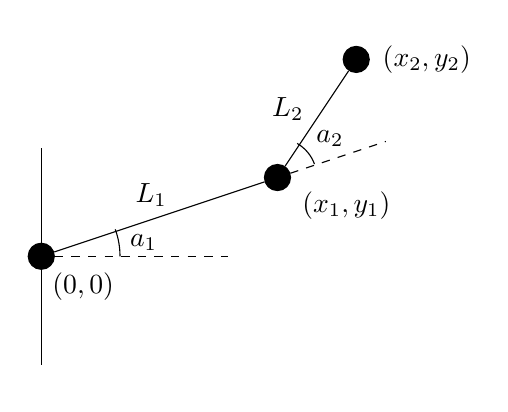
\begin{tikzpicture}[]
	%\draw[help lines] (-2,0) grid (20,10);
	
	\tikzstyle{vnode} = [circle,draw,fill=black,minimum size=1mm]
	\tikzstyle{inode} = [minimum size=8mm]
	\tikzstyle{vedge} = [->,>=latex,thick]
	
	

\node[vnode] (v1) at (-13,-1.5) {};
\node[vnode] (v2) at (-10,-0.5) {};
\node[vnode] (v3) at (-9,1) {};

\draw (v1) edge (v2);
\draw (v2) edge (v3);

\node (v5) at (-13,0) {};
\node (v4) at (-13,-3) {};
\draw  (v4) edge (v5);
\node (v6) at (-10.5,-1.5) {};
\node (v7) at (-8.5,0) {};
\draw [dashed] (v1) edge (v6);
\draw [dashed] (v2) edge (v7);

\node[inode] (a1) at (-11.7009,-1.3281) {$a_1$};
\node[inode] (a2) at (-9.3344,-0.0033) {$a_2$};

\node[inode] (a1) at (-11.6046,-0.7257) {$L_1$};
\node[inode] (a1) at (-9.8685,0.3693) {$L_2$};

\node[inode] (a1) at (-12.4679,-1.8791) {$(0, 0)$};
\node[inode] (a1) at (-9.1257,-0.8593) {$(x_1, y_1)$};
\node[inode] (a1) at (-8.1043,1.0032) {$(x_2, y_2)$};
\draw [](-12,-1.5) arc (0:20:1);
\draw [](-9.5302,-0.329) arc (20.0007:60:0.5);
\end{tikzpicture}
\end{document}
